\section{Deriving Hedin's equations}
\subsection{Time-Domain Definition of the Green's Function}
Start by considering the equation of motion for the field operators
\begin{equation}
  i\frac{\partial}{\partial t}\hat{\psi}(\mathbf{x}, t) = [\hat{\psi}(\mathbf{x}, t),\hat{H}_{elec}] = [\hat{\psi}(\mathbf{x}, t), \hat{H}_0 + \hat{H}_{int}] = [\hat{\psi}(\mathbf{x}, t), \hat{H}_0] + [\hat{\psi}(\mathbf{x}, t), \hat{H}_{int}] 
\end{equation}
For the non-interacting part, we have
\begin{align}
  [\hat{\psi}(\mathbf{x}, t), \hat{H}_0] &= [\hat{\psi}(\mathbf{x}, t), \int d\mathbf{x}' \hat{\psi}^\dagger(\mathbf{x}', t)\hat{h}^0(\mathbf{x}')\hat{\psi}(\mathbf{x}', t)] \\
  &= \int d\mathbf{x}' [\hat{\psi}(\mathbf{x}, t), \hat{\psi}^\dagger(\mathbf{x}', t)\hat{h}^0(\mathbf{x}')\hat{\psi}(\mathbf{x}', t)] \\
  &= \int d\mathbf{x}' \left( \underbrace{[\hat{\psi}(\mathbf{x}, t), \hat{\psi}^\dagger(\mathbf{x}', t)]}_{\delta(\mathbf{x}-\mathbf{x}')}\hat{h}^0(\mathbf{x}')\hat{\psi}(\mathbf{x}', t) + \hat{\psi}^\dagger(\mathbf{x}', t)\hat{h}^0(\mathbf{x}')\underbrace{[\hat{\psi}(\mathbf{x}, t), \hat{\psi}(\mathbf{x}', t)]}_{0} \right) \\
  &= h^0(\mathbf{x})\hat{\psi}(\mathbf{x}, t).
\end{align}
For the interacting part, we have
\begin{align}
 &[\hat{\psi}(\mathbf{x}, t), \hat{H}_{int}] = \frac{1}{2}\int d\mathbf{x}' d\mathbf{x}'' v(\mathbf{x},\mathbf{x}') [ \hat{\psi}(\mathbf{x}, t), \hat{\psi}^\dagger(\mathbf{x}', t)  \hat{\psi}^{\dagger}(\mathbf{x}'', t) \hat{\psi}(\mathbf{x}'', t) \hat{\psi}(\mathbf{x}', t) ] \\
&= \frac{1}{2}\int d\mathbf{x}' d\mathbf{x}'' v(\mathbf{x},\mathbf{x}') \left( \delta (\mathbf{x}-\mathbf{x}') \hat{\psi}^\dagger(\mathbf{x}'', t) \hat{\psi}(\mathbf{x}'', t) \hat{\psi}(\mathbf{x}', t) + \hat{\psi}^\dagger(\mathbf{x}', t) \delta (\mathbf{x}-\mathbf{x}'') \hat{\psi}(\mathbf{x}'', t) \hat{\psi}(\mathbf{x}', t) \right) \\
&= \int d\mathbf{x}' \hat{\psi}^\dagger(\mathbf{x}', t) v(\mathbf{x},\mathbf{x}') \hat{\psi}(\mathbf{x}', t) \hat{\psi}(\mathbf{x}, t)
\end{align}
so overall we have
\begin{equation}
  i\frac{\partial}{\partial t}\hat{\psi}(\mathbf{x}, t) = \left( \hat{h}^0(\mathbf{x}) + \int d\mathbf{x}' v(\mathbf{x},\mathbf{x}') \hat{\psi}^\dagger(\mathbf{x}', t) \hat{\psi}(\mathbf{x}', t) \right) \hat{\psi}(\mathbf{x}, t) 
\end{equation}
Now we can consider the equation of motion for the Green's function, defined as $G(\mathbf{x}t, \mathbf{x}'t') = -i \bra{N}\mathcal{T}\left(\hat{\psi}(\mathbf{x},t)\hat{\psi}^\dagger(\mathbf{x}',t')\right)\ket{N}$, where $\mathcal{T}$ is the time-ordering operator.
\begin{align}
  \frac{\partial}{\partial t}G(\mathbf{x}t, \mathbf{x}'t') &= -i \bra{N}\frac{\partial}{\partial t}\mathcal{T}\left(\hat{\psi}(\mathbf{x},t)\hat{\psi}^\dagger(\mathbf{x}',t')\right)\ket{N} \\
\end{align}
Now,
\begin{align}
  &\frac{\partial}{\partial t}\mathcal{T}\left(\hat{\psi}(\mathbf{x},t)\hat{\psi}^\dagger(\mathbf{x}',t')\right) = \frac{\partial}{\partial t}\left( \theta(t-t')\hat{\psi}(\mathbf{x},t)\hat{\psi}^\dagger(\mathbf{x}',t') - \theta(t'-t)\hat{\psi}^\dagger(\mathbf{x}',t')\hat{\psi}(\mathbf{x},t) \right) \\
  &= \underbrace{\frac{\partial \theta(t-t')}{\partial t}}_{\delta(t-t')}\hat{\psi}(\mathbf{x},t)\hat{\psi}^\dagger(\mathbf{x}',t') + \theta(t-t')\frac{\partial}{\partial t}\hat{\psi}(\mathbf{x},t)\hat{\psi}^\dagger(\mathbf{x}',t') - \underbrace{\frac{\partial \theta(t'-t)}{\partial t}}_{-\delta(t'-t)}\hat{\psi}^\dagger(\mathbf{x}',t')\hat{\psi}(\mathbf{x},t) - \theta(t'-t)\frac{\partial}{\partial t}\hat{\psi}^\dagger(\mathbf{x}',t')\hat{\psi}(\mathbf{x},t) \\
  &= \underbrace{\delta(t-t') {\acomm{\hat{\psi}(\mathbf{x},t)}{\hat{\psi}^\dagger(\mathbf{x}',t')}}}_{\delta(\mathbf{x}-\mathbf{x}') \delta(t-t')} + \mathcal{T}\left(\frac{\partial}{\partial t}\hat{\psi}(\mathbf{x},t)\hat{\psi}^\dagger(\mathbf{x}',t')\right) \\
\end{align}
So now consider plugging in the equation of motion for $\hat{\psi}(\mathbf{x},t)$ into the above expression
\begin{align}
  &\mathcal{T}\left(\frac{\partial}{\partial t}\hat{\psi}(\mathbf{x},t)\hat{\psi}^\dagger(\mathbf{x}',t')\right) = \mathcal{T}\left(-i \left( \hat{h}^0(\mathbf{x}) + \int d\mathbf{x}'' v(\mathbf{x},\mathbf{x}'') \hat{\psi}^\dagger(\mathbf{x}'',t) \hat{\psi}(\mathbf{x}'',t) \right) \hat{\psi}(\mathbf{x},t)\hat{\psi}^\dagger(\mathbf{x}',t')\right) \\
  &=  -i \hat{h}^0(\mathbf{x}) \mathcal{T}\left(\hat{\psi}(\mathbf{x},t)\hat{\psi}^\dagger(\mathbf{x}',t')\right) - i \int d\mathbf{x}'' v(\mathbf{x},\mathbf{x}'') \mathcal{T}\left(\hat{\psi}(\mathbf{x},t)\hat{\psi}^\dagger(\mathbf{x}'',t) \hat{\psi}(\mathbf{x}'',t) \hat{\psi}^\dagger(\mathbf{x}',t')\right)
\end{align}
So we have
\begin{align}
  \left[ i \frac{\partial}{\partial t} - \hat{h}^0(\mathbf{x}) \right] G(\mathbf{x}t, \mathbf{x}'t') = \delta(\mathbf{x}-\mathbf{x}') \delta(t-t') - i \int d\mathbf{x}'' v(\mathbf{x},\mathbf{x}'') \underbrace{G_2(\mathbf{x}t, \mathbf{x}''t, \mathbf{x}'t^+ , \mathbf{x}'t')}_{\bra{N}\mathcal{T}\left(\hat{\psi}(\mathbf{x},t)\hat{\psi}(\mathbf{x}'',t)\hat{\psi}^\dagger(\mathbf{x}'',t')\hat{\psi}^\dagger(\mathbf{x}',t')\right)\ket{N}}
\end{align}
and we notice that in order to compute the single-particle Green's function, we need to know the two-particle Green's function, which needs the three-particle Green's function, and so on. So to simplify we introduce a nonlocal, time-dependent self-energy $\Sigma(\mathbf{x}t, \mathbf{x}'t')$ that satisfies
\begin{align}
  - i \int d\mathbf{x}'' v(\mathbf{x}, \mathbf{x}'') G_2(\mathbf{x}t, \mathbf{x}''t, \mathbf{x}'t^+ , \mathbf{x}'t') \equiv \int dt'' \int d\mathbf{x}'' \overline{\Sigma}(\mathbf{x} t , \mathbf{x}'' t'' ) G(\mathbf{x}''t'', \mathbf{x}'t')
\end{align}
and further define $\Sigma = \overline{\Sigma} - v_H$ with
\begin{align}
  v_H(\mathbf{x},t) = \int d\mathbf{x}' v(\mathbf{x}, \mathbf{x}') \underbrace{\bra{N} \hat{\psi}^\dagger(\mathbf{x}') \hat{\psi}(\mathbf{x}') \ket{N}}_{-\frac{1}{i}G(\mathbf{x}'t, \mathbf{x}'t)} = i \int d\mathbf{x}' v(\mathbf{x}, \mathbf{x}') G(\mathbf{x}'t, \mathbf{x}'t)
  \label{eq:hartree}
\end{align}
and we can rewrite the equation of motion as
\begin{align}
  \left[ i \frac{\partial}{\partial t} - \hat{h}^0(\mathbf{x}) - v_H(\mathbf{x},t) \right] G(\mathbf{x}t, \mathbf{x}'t') = \delta(\mathbf{x}-\mathbf{x}') \delta(t-t') + \int dt'' \int d\mathbf{x}'' \Sigma(\mathbf{x}t, \mathbf{x}''t'') G(\mathbf{x}''t'', \mathbf{x}'t')
  \label{eq:eom_green}
\end{align}
Now consider defining the $G_0$ of the non-interacting system
\begin{align}
    \left[ i \frac{\partial}{\partial t} - \hat{h}^0(\mathbf{x}) - v_H(\mathbf{x},t) \right] G_0(\mathbf{x}t, \mathbf{x}'t') = \delta(\mathbf{x}-\mathbf{x}') \delta(t-t')
    \label{eq:eom_green_0}
\end{align}
So we can write equations \ref{eq:eom_green} and \ref{eq:eom_green_0} symbolically as
\begin{align}
  \hat{O} G &= \delta + \Sigma G \quad \text{and} \quad \hat{O} G_0 = \delta \\
  &\implies G_0 = \hat{O}^{-1} \implies G = G_0 + G_0 \Sigma G \\
  &\implies G(1,2) = G_0(1,2) + \int d3 d4 G_0(1,3) \Sigma(3,4) G(4,2)
\end{align}
where we use the space-time notation $1 = (\mathbf{x}_1,t_1)$ etc.

\subsection{Hedin's Equations}
Schwinger chose to introduce a potential $\varphi$ that we will later set to zero, in order to rewrite the two-particle Green's function as
\begin{equation}
  G_2(1,3,2,3^+) = G(1,2) \, G(3,3^+) - \frac{\delta G(1,2)}{\delta \varphi(3)},
  \label{eq:schwinger}
\end{equation}
So
\begin{align}
  \bar{\Sigma}(1,2) &= -i \int d(3) \; v(1,3)\, G_2(1,3,2,3^+) \\
  &= -i \int d(3)\, v(1,3) \left[ G(1,2)\, G(3,3^+) - \frac{\delta G(1,2)}{\delta \varphi(3)} \right] \\
  &= -i\, G(1,2) \underbrace{\int d(3)\, v(1,3)\, G(3,3^+)}_{-i v_H(1)} + i \int d(3)\, v(1,3)\, \frac{\delta G(1,2)}{\delta \varphi(3)}.
  \label{eq:sigma_intermediate}
\end{align}
Now because $\delta G = -G  \left( \delta G^{-1} \right) G$ we can write the identity
\begin{equation}
  \frac{\delta G(1,2)}{\delta \varphi(3)} = - \int d(4)d(5) \; G(1,4) \, \frac{\delta G^{-1}(4,5)}{\delta \varphi(3)} \, G(5,2).
  \label{eq:deltaG}
\end{equation}
So the second term in Eq.~\eqref{eq:sigma_intermediate} gives
\begin{align}
  i\int d(3)\; v(1,3)\, \frac{\delta G(1,2)}{\delta \varphi(3)}
  &= -i \int d(3) \, v(1,3) \int d(4)d(5) \; G(1,4) \, \frac{\delta G^{-1}(4,5)}{\delta \varphi(3)} \, G(5,2) \nonumber \\
  &= -i \int d(3,4,5) \; v(1,3)\, G(1,4)\, \frac{\delta G^{-1}(4,5)}{\delta \varphi(3)}\, G(5,2).
  \label{eq:second_term}
\end{align}
Now we can get rid of a \(G(1,2)\) dependence by multiplying with \(G^{-1}\), yielding
\begin{equation}
  \overline{\Sigma}(1,2) = -\delta(1,2)\,v_H(1) -i\int d(3,4)\; v(1,3)\, G(1,4)\, \frac{\delta G^{-1}(4,2)}{\delta \varphi(3)}.
  \label{eq:sigma_final}
\end{equation}
Introduce $V(1) = \varphi(1) + v_H(1)$ as the total potential that electrons experience. Consider
\begin{equation}
  \frac{\delta G^{-1}(1,2)}{\delta \varphi(3)} \equiv \underbrace{\frac{\delta G^{-1}(1,2)}{\delta V(5)}}_{-\Gamma(1,2,5)} \underbrace{\frac{\delta V(5)}{\delta \varphi(3)}}_{\varepsilon^{-1}(5,3)}.
  \label{eq:deltaG_V}
\end{equation}
So
\begin{align}
  \overline{\Sigma}(1,2) = -\delta(1,2)\,v_H(1) +i\int d(5) \underbrace{\int d(3) v(1,3)\, \varepsilon^{-1}(3,5)}_{W(1,5 )}\, \int d(4) G(1,4)\, \Gamma(4,5,2).
  \label{eq:sigma_final_2}
\end{align}
and if we further make the GW approximation where $\Gamma(4,5,2) \approx \delta(4,5)\delta(2,5)$ we get
\begin{equation}
  \overline{\Sigma}(1,2)  = -\delta(1,2)\,v_H(1) + iW(1,2) G(1,2)
  \label{eq:sigma_final_3}
\end{equation}
and if we just care about the exchange-correlation part, we can define
\begin{align}
   {\Sigma}_{xc}(1,2) = \overline{\Sigma}(1,2) + \delta(1,2)\,v_H(1) = i W(1,2) G(1,2) \implies \Sigma_{xc}(\tau) = i W(\tau) G(\tau)
  \label{eq:sigma_xc}
\end{align}
where $\tau = t_1 - t_2$. Define $G(\tau) = \int \frac{d\omega'}{2\pi} e^{-i\omega'\tau} G(\omega')$ and $W(\tau) = \int \frac{d\omega''}{2\pi} e^{-i\omega''\tau} W(\omega'')$ to get
\begin{equation}
  \Sigma_{xc}(\tau) = i \int \frac{d\omega'}{2\pi} \int \frac{d\omega''}{2\pi} e^{-i(\omega'+\omega'')\tau} G(\omega') W(\omega'')
  \label{eq:sigma_xc_freq}
\end{equation}
Taking the inverse Fourier transform of $\Sigma_{xc}(\tau)$ we get
\begin{equation}
  \Sigma_{xc}(\omega) = \int \frac{d\tau}{2\pi} e^{i\omega\tau} \Sigma_{xc}(\tau) = i \int \frac{d\omega'}{2\pi} \int \frac{d\omega''}{2\pi} G(\omega') W(\omega'') \underbrace{\int d\tau  e^{i(\omega -\omega'-\omega'')\tau}}_{2\pi \delta(\omega -\omega'-\omega'')} = i \int \frac{d\omega'}{2\pi} G(\omega') W(\omega-\omega')
  \label{eq:sigma_xc_inv_freq}
\end{equation}
Now in $G_0W_0$ one applies the Cauchy residue theorem to solve this convolution integral, yielding
the known form.





\section{Final expressions}
\subsection{Fully analytic}
I follow the notation of Tianyu's paper throughout this section \cite{Zhu2020-nt}.
    We want to solve for the self-energy whose form along the real axis is:
    \begin{equation}
    \Sigma\left(\mathbf{r}, \mathbf{r}^{\prime}, \omega\right)=\frac{i}{2 \pi} \int_{-\infty}^{\infty} e^{i\omega ^{\prime}\eta }d \omega^{\prime} G_{0}\left(\mathbf{r}, \mathbf{r}^{\prime}, \omega+\omega^{\prime}\right) W_{0}\left(\mathbf{r}, \mathbf{r}^{\prime}, \omega^{\prime}\right)
    \end{equation}
    In the molecular brutal basis, the self energy is given as:
    \begin{equation}
        \Sigma_{n n^\prime}(\mathbf{k}, \omega) = \iint d \mathbf{r} d \mathbf{r}^\prime \psi_{n\mathbf{k}}^{*}(\mathbf{r}) \Sigma(\mathbf{r}, \mathbf{r}^\prime, \omega) \psi_{n^\prime\mathbf{k}}(\mathbf{r}^\prime)
    \end{equation}
    Also, recall that the Lehmann representation of the noninteracting Green's function is:
    \begin{equation}
        G_0\left(\mathbf{r}, \mathbf{r}^{\prime}, \omega\right)=\sum_{o \mathbf{q} } \frac{\psi_{o \mathbf{q}}(\mathbf{r}) \psi_{o \mathbf{q}}^{*}\left(\mathbf{r}^{\prime}\right)}{\omega-\epsilon_{o \mathbf{q}}+i \eta \operatorname{sgn}\left(\epsilon_{o \mathbf{q}}-\mu\right)}
    \end{equation}
    Now plugging both of these back into the original expression, we find:


    \begin{align}
        \Sigma_{n n^\prime}(\mathbf{k}, \omega) &= \frac{i}{2 \pi} \sum_{o \mathbf{q}} \int_{-\infty}^{\infty} d \omega^{\prime} \frac{e^{i\omega ^{\prime}\eta }}{\omega + \omega^{\prime} - \epsilon_{o \mathbf{q}} + i \eta \operatorname{sgn}\left(\epsilon_{o \mathbf{q}}-\mu\right)} \nonumber \\
        &\quad \times \iint d \mathbf{r} d \mathbf{r}^\prime \psi_{n\mathbf{k}}^{*}(\mathbf{r}) \psi_{o \mathbf{q}}(\mathbf{r}) W_0(\mathbf{r}, \mathbf{r}^\prime, \omega^{\prime}) \psi_{o \mathbf{q}}^{*}\left(\mathbf{r}^{\prime}\right) \psi_{n^\prime\mathbf{k}}(\mathbf{r}^\prime)\\
        &= \frac{i}{2 \pi} \sum_{o \mathbf{q}} \int_{-\infty}^{\infty} d \omega^{\prime} \frac{e^{i\omega ^{\prime}\eta }}{\omega + \omega^{\prime} - \epsilon_{o \mathbf{k}-\mathbf{q}} + i \eta \operatorname{sgn}\left(\epsilon_{o \mathbf{k}-\mathbf{q}}-\mu\right)} (n_{\mathbf{k}}o_{\mathbf{k-q}}|W_0|o_{\mathbf{k-q}}n^\prime_{\mathbf{k}})
    \end{align}
    Where we have used the fact that the momentum index $\mathbf{q}$ is the same as $\mathbf{k}-\mathbf{q}$, given that we are looping over both $\mathbf{k}$ and $\mathbf{q}$ anyways.


    So the Green's function will bring poles at \(\omega' = \epsilon_{0 \mathbf{k-q}} - \omega+ i\eta\operatorname{sgn}(\mu - \epsilon_{0 \mathbf{k-q}})\).
    Now, we know that the screened Coulomb interaction has the expansion in terms of the bare Coulomb potential \(v\) and the density response function \(\chi_0\) as \(W_0 = v + v\chi_0 v + v\chi_0 v\chi_0 v + \cdots = v\left(1 + \chi_0 v + \chi_0 v \chi_0 v + \cdots\right) = v\left(1 - \chi_0 v\right)^{-1}\), where we recognize the dielectric function as \(\epsilon_0 = 1 - \chi_0 v\) so we can express the screened Coulomb interaction as
    \begin{equation}
    W_0(\mathbf{r}, \mathbf{r}^{\prime}, \omega) = \frac{v(\mathbf{r}, \mathbf{r}^{\prime})}{1 - \left(\chi_0v\right)(\mathbf{r}, \mathbf{r}^{\prime}, \omega)}
    \end{equation}
    recalling that the bare Coulomb interaction should be independent of frequency. A discussion of how to compute the screened Coulomb interaction can be found in this old work \cite{Onida2002-pw}. To simplify notation let us define a polarizability $\boldsymbol{\Pi}\left(\mathbf{r}, \mathbf{r}^{\prime}, \omega\right) = \left(\chi_0 v\right)(\mathbf{r}, \mathbf{r}^{\prime}, \omega)$, so that we can rewrite the screened Coulomb interaction as:
\begin{align}
    (n_{\mathbf{k}}o_{\mathbf{k-q}}|W_0|o_{\mathbf{k-q}}n^\prime_{\mathbf{k}}) = \iint d \mathbf{r} d \mathbf{r}^\prime \psi_{n\mathbf{k}}^{*}(\mathbf{r}) \psi_{o \mathbf{q}}(\mathbf{r}) W_0(\omega ) \psi_{o \mathbf{q}}^{*}\left(\mathbf{r}^{\prime}\right) \psi_{n^\prime\mathbf{k}}(\mathbf{r}^\prime)
\end{align}
At this point, we recognize the decomposition of the ERIs with the Cholesky vectors as:
\begin{equation}
    (p_{\mathbf{k}_p} q_{\mathbf{k}_q} |\frac{1}{|\mathbf{r}-\mathbf{r}^\prime|} |r_{\mathbf{k}_r} s_{\mathbf{k}_s}) = \sum_{PQ} v_{P{\mathbf{q}}}^{p\mathbf{k_p}q\mathbf{k_q}} v_{Q{(\mathbf{-q})}}^{r\mathbf{k_r}s\mathbf{k_s}}
\end{equation}
so each Cholesky brings a factor of $\mathbf{J}^{\frac{1}{2}}$. Each Cholesky is defined as:
\begin{equation}
    v_{P{\mathbf{q}}}^{p\mathbf{k_p}q\mathbf{k_q}} = \sum_{R} \mathbf{J}_{RP}^{-\frac{1}{2}}(\mathbf{q}) \left(R \mathbf{q} \mid p \mathbf{k}_p q \mathbf{k}_q\right)
\end{equation}
where
\begin{equation}
\begin{aligned}
\mathbf{J}_{PQ}(\mathbf{k}) & =\iint d \mathbf{r} d \mathbf{r}^{\prime} \phi_{P(-\mathbf{k})}(\mathbf{r}) \frac{1}{\left|\mathbf{r}-\mathbf{r}^{\prime}\right|} \phi_{Q \mathbf{k}}\left(\mathbf{r}^{\prime}\right) \\
\left(Q \mathbf{k}_{r s} \mid r \mathbf{k}_r s \mathbf{k}_s\right) & =\iint d \mathbf{r} d \mathbf{r}^{\prime} \phi_{Q \mathbf{k}_{r s}}(\mathbf{r}) \frac{1}{\left|\mathbf{r}-\mathbf{r}^{\prime}\right|} \phi_{r \mathbf{k}_r}^*\left(\mathbf{r}^{\prime}\right) \phi_{s \mathbf{k}_s}\left(\mathbf{r}^{\prime}\right)
\end{aligned}
\end{equation}
So the simplest thing now will be to derive an expression for the columb interaction in terms of an auxiliary basis:
\begin{equation}
W_{0, PQ}(\omega)=\left[\mathbf{J}(\mathbf{I}-\mathbf{\Pi}(\mathbf{q}, \omega))^{-1}\right]_{PQ}
\end{equation}
and then we need to contract with the Choleskies to get the matrix element:
\begin{equation}
    (n_{\mathbf{k}}o_{\mathbf{k-q}}|W_0|o_{\mathbf{k-q}}n^\prime_{\mathbf{k}}) =\sum_{PQ} v_{P}^{nm}\left[\mathbf{I}-\mathbf{\Pi}\left(\mathbf{q}, \omega\right)\right]_{PQ}^{-1} v_{Q}^{mn^{\prime}}
\end{equation}

So in our quest to find poles of $W_0$, we are really just looking for poles of the $\chi_0$. $\chi_0$ is given by:
\begin{equation}
\chi_{0}\left(\mathbf{r}, \mathbf{r}^{\prime}, \omega\right)=\sum_{r\mathbf{k} s \mathbf{k}^{\prime}}\left(f_{r \mathbf{k}}-f_{s \mathbf{k}^{\prime}}\right) \frac{\psi_{r \mathbf{k}}(\mathbf{r}) \psi_{r \mathbf{k}}^{*}\left(\mathbf{r}^{\prime}\right) \psi_{s \mathbf{k}^{\prime}}\left(\mathbf{r}^{\prime}\right) \psi_{s \mathbf{k}^{\prime}}^{*}(\mathbf{r})}{\omega-\left(\epsilon_{r \mathbf{k}}-\epsilon_{s \mathbf{k}^{\prime}}\right)+i \eta \operatorname{sgn}\left(\epsilon_{r \mathbf{k}}-\epsilon_{s \mathbf{k}^{\prime} } - \mu\right)}
\end{equation}
where the occupations of the KS states \(r\mathbf{k}(s\mathbf{k}^{\prime})\) with energies \(\epsilon_{r\mathbf{k}}(\epsilon_{s\mathbf{k}^{\prime}})\) are given by the Fermi-Dirac distribution \(f_{r\mathbf{k}}(f_{s\mathbf{k}^{\prime}})\), which is just a step function at zero temperature. Notice that the occupation factor will always be 0 unless \(rs\) form an occupied-virtual pair. So we can separate the density response into two terms, one where \(\delta_{ri}\) and \(\delta_{sa}\) and the other with \(\delta_{ra}\) and \(\delta_{si}\), where \(i\) and \(a\) are occupied and virtual indices, respectively. This allows us to now combine with the bare Coulomb potential in order to form the polarizability \(\Pi\equiv \chi_0v\) as:
\begin{equation}
\Pi\left(\mathbf{r}, \mathbf{r}^{\prime}, \omega\right)=\sum_{i\mathbf{k}a\mathbf{k}^{\prime}}\frac{\psi_{i\mathbf{k}}(\mathbf{r}) \psi_{i\mathbf{k}}^{*}\left(\mathbf{r}^{\prime}\right)\frac{1}{|\mathbf{r}-\mathbf{r}^\prime|} \psi_{a\mathbf{k}^{\prime}}\left(\mathbf{r}^{\prime}\right) \psi_{a\mathbf{k}^{\prime}}^{*}(\mathbf{r})}{\omega+\left(\Omega_{i\mathbf{k}a\mathbf{k}^{\prime}}\right)-i\eta } - \sum_{a\mathbf{k}i\mathbf{k}^{\prime}}\frac{\psi_{a\mathbf{k}}(\mathbf{r}) \psi_{a\mathbf{k}}^{*}\left(\mathbf{r}^{\prime}\right) \frac{1}{|\mathbf{r}-\mathbf{r}^\prime|}\psi_{i\mathbf{k}^{\prime}}\left(\mathbf{r}^{\prime}\right) \psi_{i\mathbf{k}^{\prime}}^{*}(\mathbf{r})}{\omega-\left(\Omega_{i\mathbf{k}a\mathbf{k}^{\prime}}\right)+i\eta },
\end{equation}
where we define the KS eigenvalue differences as \(\Omega_{i\mathbf{k}a\mathbf{k}^{\prime}} = \epsilon_{a\mathbf{k}} - \epsilon_{i\mathbf{k}^{\prime}}\), which will eventually become the excitation energies from RPA. So sandwiching this operator in between the molecular or brutal bases gives:
\begin{equation}
    \bra{n\mathbf{k}} \Pi (\omega) \ket{n^\prime\mathbf{k}} = \sum_{iajb \mathbf{k} \mathbf{k}^{\prime}} \frac{(ia\mid jb)}{(\omega + \Omega ^{\mu}_{\mathbf{k}})-i\eta} - \sum_{aibj \mathbf{k} \mathbf{k}^{\prime}} \frac{(ai\mid bj)}{(\omega - \Omega ^{\mu}_{\mathbf{k}})+i\eta}
\end{equation}
\emph{So we see that we can get the poles of the screened Coulomb interaction by the poles of the polarizability, which are \(\omega = \Omega ^{\mu}_{\mathbf{k}} - i\eta\) and \(\omega = \Omega ^{\mu}_{\mathbf{k}} + i\eta\), suggesting that they are in the upper complex plane for excitations and vice versa for deexcitations.} See the figure \ref{fig:contour} for a picture. For a more comprehensive picture, this should be juxtaposed with the figure from Tianyu's paper for CD. In the literature, they talk about approximating the dielectric function by a multiple one or a single pole approximation, so which one would I want to implement? This suggests that the notation in the \(G_0W_0\) literature is confusing because they always say that to solve for the \(\chi_0\) in the RPA, but if we are actually dealing with \(\chi_0\), which is the Kohn-Sham density response function, then we don't use the RPA, where the density response function is solved for using a Dyson-like equation \cite{Sander2015-xq}:
    \begin{figure}[h]
    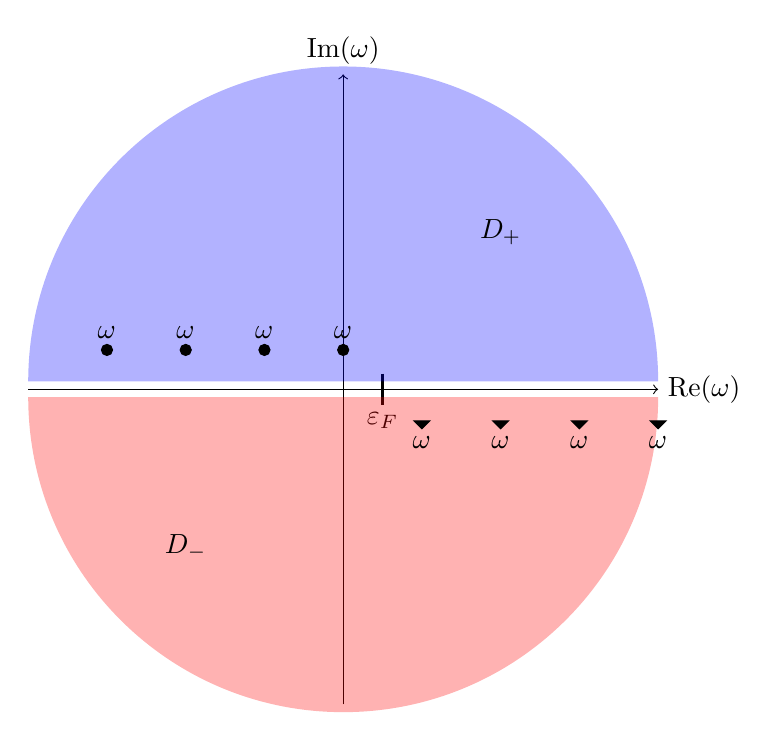
\begin{tikzpicture}
    % Draw the axes
    \draw[->] (-4, 0) -- (4, 0) node[right] {Re($\omega$)};
    \draw[->] (0, -4) -- (0, 4) node[above] {Im($\omega$)};
    
    % Draw the positive real axis label and tick mark for \varepsilon_{F}
    \draw[thick] (0.5, 0.2) -- (0.5, -0.2);
    \node at (0.5, -0.4) {$\varepsilon_{F}$};


    % Draw the semicircle contours
    % fill in its under side
    \fill[blue, opacity=0.3] (4, 0.1) arc[start angle=0, end angle=180, radius=4];
    \fill[red, opacity=0.3] (4, -0.1) arc[start angle=0, end angle=-180, radius=4];
    
    % Draw the poles above the real axis
    \foreach \x in {-3,-2,-1,0} {
        \draw[fill=black] (\x, 0.5) circle (2pt);
    }
    \node at (-3, 0.7) {$\omega_{}$};
    \node at (-2, 0.7) {$\omega_{}$};
    \node at (-1, 0.7) {$\omega_{}$};
    \node at (0, 0.7) {$\omega_{}$};    

    % Draw the poles below the real axis
    \foreach \x in {1,2,3,4} {
        \draw[fill=black] (\x, -0.5) -- ++(0.1, 0.1) -- ++(-0.2, 0) -- cycle;
    }
    \node at (1, -0.7) {$\omega_{}$};
    \node at (2, -0.7) {$\omega_{}$};
    \node at (3, -0.7) {$\omega_{}$};
    \node at (4, -0.7) {$\omega_{}$};

    
    % Label the contours
    \node at (2, 2) {$D_+$};
    \node at (-2, -2) {$D_-$};
    \end{tikzpicture}
    \caption{Contour for the complex frequency integral. The poles are denoted by the various $\omega$. The Fermi energy is denoted by $\varepsilon_F$. The integration contour $D_+$ is the semicircle in the upper complex plane, while $D_-$ is the semicircle in the lower complex plane.}
    \label{fig:contour}
    \end{figure}
\begin{equation}\label{eq:dyson}
    \chi^{\lambda}\left(\mathbf{r}, \mathbf{r}^{\prime}, i \omega\right) = \chi^{0}\left(\mathbf{r}, \mathbf{r}^{\prime}, i \omega\right) 
    + \int d \mathbf{r}_{1} d \mathbf{r}_{2} \chi^{0}\left(\mathbf{r}, \mathbf{r}_{1}, i \omega\right)\left[\frac{\lambda}{\left|\mathbf{r}_{1}-\mathbf{r}_{2}\right|}+f_{\mathrm{xc}}^{\lambda}\left(\mathbf{r}_{1}, \mathbf{r}_{2}, i \omega\right)\right] \chi^{\lambda}\left(\mathbf{r}_{2}, \mathbf{r}^{\prime}, \omega\right)
\end{equation}
where the parameter $\lambda$ controls the amount of interaction in the system, ranging from $\lambda = 0$ for the KS reference system to $\lambda = 1$ for the fully interacting system. The $f_{\mathrm{xc}}^{\lambda}$ is the exchange-correlation kernel, which is set to zero for the RPA. But we will proceed with an RPA calculation anyways in order to solve for the excitation energies and their corresponding eigenvectors. So it makes sense that the numerator of the expression for the screened Coulomb interaction should be given a construction of the ERIs with the excitation factors in a transition density defined as:
\begin{equation}
    w_{pq}^{\mu} = \sum_{ia} (pq|ia) \left(X_{ia}^{\mu} + Y_{ai}^{\mu}\right)
\end{equation}
where we have defined the excitation and de-excitation vectors at the excitation index $\mu$ as $X_{ia}^{\mu}$ and $Y_{ai}^{\mu}$, respectively.
I am not sure how to connect this with the known expression $v\epsilon ^{-1}$; I see the similarities given that we are contracting an ERI with what we get from the RPA calculation that is connected to the polarizability, but can't connect exactly.
We want to figure out how this matches with my previous $O(N^6)$ expression, which was
\begin{equation}
    \Sigma_{pp}^{\text{corr}}(\omega) = \sum_{\mu }^{\text{RPA}}\left(\sum_{i}^{\text{occupied}} \frac{w_{pi}^{\mu }w_{ip}^{\mu }}{\omega -(\epsilon _{i}-\Omega  _{\mu })}+ \sum_{a}^{\text{virtual}} \frac{w_{pa}^{\mu }w_{ap}^{\mu }}{\omega -(\epsilon _{a}+\Omega  _{\mu })}\right)
\end{equation}
for the molecular case. Today I want us to dissect how this equation came about, so that I can understand for my k-point version.
% The expression I get adapted for k-points from GPT is:
% \begin{equation}
% \Sigma_{n n^\prime}^{\text {corr }}(\mathbf{k}, \omega)=\sum_{\mathbf{q}} \sum_\mu^{\text {RPA }}\left(\sum_i^{\text {occupied }} \frac{w_{n i}^\mu(\mathbf{k}, \mathbf{q}) w_{i n^\prime}^\mu(\mathbf{k}-\mathbf{q}, \mathbf{q})}{\omega-\left(\epsilon_{i, \mathbf{k}-\mathbf{q}}-\Omega_{\mu, \mathbf{q}}\right)}+\sum_a^{\text {virtual }} \frac{w_{n a}^\mu(\mathbf{k}, \mathbf{q}) w_{a n^\prime}^\mu(\mathbf{k}-\mathbf{q}, \mathbf{q})}{\omega-\left(\epsilon_{a, \mathbf{k}-\mathbf{q}}+\Omega_{\mu, \mathbf{q}}\right)}\right)
% \end{equation}

\subsection{Analytic continuation}
\label{sec:analytic_continuation}
We start with the original form for the self-energy along the real axis:
\begin{equation}
\Sigma\left(\mathbf{r}, \mathbf{r}^{\prime}, \omega\right)=\frac{i}{2 \pi} \int_{-\infty}^{\infty} d \omega^{\prime} e^{i \omega^{\prime} \eta} G_{0}\left(\mathbf{r}, \mathbf{r}^{\prime}, \omega+\omega^{\prime}\right) W_{0}\left(\mathbf{r}, \mathbf{r}^{\prime}, \omega^{\prime}\right)
\end{equation}
But to avoid the poles, we need to evaluate along the imaginary axis, so the problem becomes:
\begin{equation*}
\Sigma\left(\mathbf{r}, \mathbf{r}^{\prime}, i \omega\right)=-\frac{1}{2 \pi} \int_{-\infty}^{\infty} d \omega^{\prime} G_{0}\left(\mathbf{r}, \mathbf{r}^{\prime}, i \omega+i \omega^{\prime}\right) W_{0}\left(\mathbf{r}, \mathbf{r}^{\prime}, i \omega^{\prime}\right) 
\end{equation*}
We are interested in evaluating the matrix elements of this operator in the molecular orbital basis. Note that both molecular orbitals must have the same crystal momentum in order for it to be conserved in this process. We also apply the identity operator:
\begin{equation}
\bra{n\mathbf{k}} \Sigma (i \omega) \ket{n^\prime\mathbf{k}} = -\frac{1}{2 \pi} \sum_{m\mathbf{k}^\prime}\int_{-\infty}^{\infty} d \omega^{\prime} \bra{n\mathbf{k}} G_0(i \omega + i \omega^{\prime}) \ket{m\mathbf{k^\prime}}\bra{m\mathbf{k^\prime}}W_0(i \omega^{\prime}) \ket{n^\prime\mathbf{k}}
\end{equation}
The noninteracting Green's function has the form:
\begin{equation*}
G_{0}\left(\mathbf{r}, \mathbf{r}^{\prime}, i \omega\right)=\sum_{m \mathbf{k}_{m}} \frac{\psi_{m \mathbf{k}_{m}}(\mathbf{r}) \psi_{m \mathbf{k}_{m}}^{*}\left(\mathbf{r^\prime}\right)}{i \omega+\epsilon_{F}-\epsilon_{m \mathbf{k}_{m}}} \implies G_{0}\left(\mathbf{k} - \mathbf{q}, i \omega + i \omega^{\prime}\right) = \sum_{m \mathbf{k}-\mathbf{q}} \frac{\psi_{m \mathbf{k}-\mathbf{q}} \psi_{m \mathbf{k}-\mathbf{q}}^{*}}{i \left(\omega + \omega^{\prime}\right) + \epsilon_{F} - \epsilon_{m \mathbf{k}-\mathbf{q}}}
\end{equation*}
so that the above equation simplifies to:
\begin{equation}
\boldsymbol{\Sigma}_{n n^{\prime}}(\mathbf{k}, i \omega) = -\frac{1}{2 \pi N_{\mathbf{k}}} \sum_{m \mathbf{q}} \int_{-\infty}^{\infty} d \omega^{\prime} \frac{(n\mathbf{k}, m\mathbf{k}-\mathbf{q} \mid W_0 (\mathbf{q}, i\omega )\mid m \mathbf{k}-\mathbf{q}, n^{\prime}\mathbf{k})}{i \left(\omega + \omega^{\prime}\right) + \epsilon_{F} - \epsilon_{m \mathbf{k}-\mathbf{q}}}
\end{equation}
\subsubsection{Screened Coulomb Interaction}
\begin{align*}
\left(n\mathbf{k}, m\mathbf{k}-\mathbf{q}\left|W_{0}(\mathbf{q}, i\omega )\right| m\mathbf{k}-\mathbf{q}, n^{\prime}\mathbf{k}\right) &= \int \int d \mathbf{r}_1 d \mathbf{r}_2 \psi_{n\mathbf{k}}^{*}(\mathbf{r}_1) \psi_{m\mathbf{k}-\mathbf{q}}(\mathbf{r}_1) W_0(\mathbf{q}, \mathbf{r}_1, \mathbf{r}_2, i\omega ) \psi_{m\mathbf{k}-\mathbf{q}}^{*}(\mathbf{r}_2) \psi_{n^{\prime}\mathbf{k}}(\mathbf{r}_2) \\
\end{align*}
We expand the orbital pair product $\psi_{n \mathbf{k}}^{*}(\mathbf{r}) \psi_{m \mathbf{k}-\mathbf{q}}(\mathbf{r})$ in the auxiliary basis

\begin{equation*}
\psi_{n \mathbf{k}}^{*}(\mathbf{r}) \psi_{m \mathbf{k}-\mathbf{q}}(\mathbf{r})=\sum_{P} b_{P \mathbf{q}}^{n \mathbf{k}, m \mathbf{k}-\mathbf{q}} \phi_{P \mathbf{q}}(\mathbf{r}) 
\end{equation*}
and
\begin{equation}
    \psi_{m\mathbf{k}-\mathbf{q}}^{*}(\mathbf{r}) \psi_{n^{\prime}\mathbf{k}}(\mathbf{r}) = \sum_{Q} b_{Q(-\mathbf{q})}^{m\mathbf{k}-\mathbf{q}, n^{\prime}\mathbf{k}} \phi_{Q(-\mathbf{q})}(\mathbf{r})
\end{equation}
where we have recognized the fact that in the former there is a momentum transfer of $\mathbf{q}$, and in the latter, there is a momentum transfer of $-\mathbf{q}$.
Substituting in gives
\begin{align}
    \left(n\mathbf{k}, m\mathbf{k}-\mathbf{q}\left|W_{0}(\mathbf{q}, i\omega )\right| m\mathbf{k}-\mathbf{q}, n^{\prime}\mathbf{k}\right)\\ = \sum_{PQ} b_{P\mathbf{q}}^{n\mathbf{k}, m\mathbf{k}-\mathbf{q}} \left[\iint d\mathbf{r}_1 d\mathbf{r}_2 \phi_{P\mathbf{q}}(\mathbf{r}_1) W_0(\mathbf{q}, \mathbf{r}_1, \mathbf{r}_2, i\omega ) \phi_{Q(-\mathbf{q})}(\mathbf{r}_2)\right] b_{Q(-\mathbf{q})}^{m\mathbf{k}-\mathbf{q}, n^{\prime}\mathbf{k}}
\end{align}
with

\begin{equation}
b_{P \mathbf{q}}^{n \mathbf{k}, m \mathbf{k}-\mathbf{q}}=\sum_{R}(n \mathbf{k}, m \mathbf{k}-\mathbf{q} \mid R \mathbf{q}) \cdot \mathbf{J}_{R P}^{-1}(\mathbf{q})
\label{eq:nonchol}
\end{equation}
Now is a good place to recall their definition of the density fitting where the ERIs are represented as:


\begin{equation*}
\left(p \mathbf{k}_{p} q \mathbf{k}_{q} \mid r \mathbf{k}_{r} s \mathbf{k}_{s}\right)=\sum_{P Q}\left(p \mathbf{k}_{p} q \mathbf{k}_{q} \mid P \mathbf{k}_{p q}\right) \mathbf{J}_{P Q}^{-1}\left(Q \mathbf{k}_{r s} \mid r \mathbf{k}_{r} s \mathbf{r}_{s}\right), 
\end{equation*}
with
\begin{align*}
\mathbf{J}_{P Q}(\mathbf{k}) & =\iint d \mathbf{r} d \mathbf{r}^{\prime} \phi_{P(-\mathbf{k})}(\mathbf{r}) \frac{1}{\left|\mathbf{r}-\mathbf{r}^{\prime}\right|} \phi_{Q \mathbf{k}}\left(\mathbf{r}^{\prime}\right),  \\
\left(Q \mathbf{k}_{r s} \mid r \mathbf{k}_{r} s \mathbf{k}_{s}\right) & =\iint d \mathbf{r} d \mathbf{r}^{\prime} \phi_{Q \mathbf{k}_{r s}}(\mathbf{r}) \frac{1}{\left|\mathbf{r}-\mathbf{r}^{\prime}\right|} \phi_{r \mathbf{k}_{r}}^{*}\left(\mathbf{r}^{\prime}\right) \phi_{s \mathbf{k}_{s}}\left(\mathbf{r}^{\prime}\right) . 
\end{align*}
Note that these $b$ are then not yet our Cholesky vectors, since each one contains $\frac{|\mathbf{r}-\mathbf{r}^{\prime}|}{|\mathbf{r}-\mathbf{r}^{\prime}|}$ scaling, i.e., there should be a factor of $\mathbf{J}^{-\frac{1}{2}}$  instead of $\mathbf{J}^{-1}$ in \ref{eq:nonchol} if we are to apply the Cholesky vectors.
At this point, we use the expansion of the screened Coulomb interaction:
\begin{align}
    W_0 &= v + v\chi_0 v + v\chi_0 v\chi_0 v + \cdots\\
    &= v(1 + \chi_0 v + \chi_0 v \chi_0 v + \cdots)\\
    &= v^{1/2} \left(1 - \chi_0\right)^{-1} v^{1/2}
\end{align}
simplifying to 
\begin{align}
    \left(n\mathbf{k}, m\mathbf{k}-\mathbf{q}\left|W_{0}(\mathbf{q}, i\omega )\right| m\mathbf{k}-\mathbf{q}, n^{\prime}\mathbf{k}\right) &= \sum_{PQ} b_{P\mathbf{q}}^{n\mathbf{k}, m\mathbf{k}-\mathbf{q}} \left[\mathbf{J^{\frac{1}{2}}}\left( \mathbf{I} - \boldsymbol{\Pi}(\mathbf{q}, i\omega ) \right) \mathbf{J^{\frac{1}{2}}}\right]^{-1}_{PQ} b_{Q(-\mathbf{q})}^{m\mathbf{k}-\mathbf{q}, n^{\prime}\mathbf{k}}\\
    &= \sum_{PQ} v_{P}^{n m}\left[\mathbf{I}-\mathbf{\Pi}\left(\mathbf{q}, i \omega^{\prime}\right)\right]_{P Q}^{-1} v_{Q}^{m n^{\prime}}
\end{align}
where $\mathbf{J}_{PQ}$ is the Coulomb interaction projected onto the auxiliary basis, and we have defined
\begin{equation}
    v_{P\mathbf{q}}^{n \mathbf{k}, m \mathbf{k}-\mathbf{q}} = \sum_{pq} C_{pn}(\mathbf{k}) C_{qm}(\mathbf{k}-\mathbf{q}) v_{P\mathbf{q}}^{p\mathbf{k}, q\mathbf{k}-\mathbf{q}}
\label{eq:mochol}
\end{equation}
with
\begin{equation}
    v_{P\mathbf{q}}^{p\mathbf{k}, q\mathbf{k}-\mathbf{q}} = \sum_R (p\mathbf{k}, q\mathbf{k}-\mathbf{q} \mid R\mathbf{q}) \mathbf{J}_{RP}^{-1/2}(\mathbf{q})
\end{equation}
If we first rename $\mathbf{k^\prime} = \mathbf{k}-\mathbf{q} \implies \mathbf{k} = \mathbf{k^\prime} + \mathbf{q}$, and then we are free to redefine $\mathbf{q} \rightarrow -\mathbf{q}$, so that \ref{eq:mochol} becomes
\begin{equation}
    v_{P\mathbf{-q}}^{n \mathbf{k}-\mathbf{q}, m \mathbf{k}} = \sum_{pq} C_{pn}(\mathbf{k}-\mathbf{q}) C_{qm}(\mathbf{k}) v_{P\mathbf{-q}}^{p\mathbf{k}-\mathbf{q}, q\mathbf{k}}
\end{equation}
but we know that the bare Coulomb potential projected onto the auxiliary basis is given by
\begin{equation}
    v_{P\mathbf{q}}^{n\mathbf{k}, m\mathbf{k}-\mathbf{q}} = \sum_{pq} C_{pn}(\mathbf{k}) C_{qm}(\mathbf{k}-\mathbf{q}) v_{P\mathbf{q}}^{p\mathbf{k}, q\mathbf{k}-\mathbf{q}}
\end{equation}

To ease notation, some momentum labels are suppressed in the above and following equations (e.g., we will use $b_{P}^{n m}$ to denote $b_{P \mathbf{q}}^{n \mathbf{k}, m \mathbf{k}-\mathbf{q}}$ ). Using Eqs. 19-21, the matrix elements of $W_{0}$ are computed as

\begin{align*}
& \left(n \mathbf{k}, m \mathbf{k}-\mathbf{q}\left|W_{0}\right| m \mathbf{k}-\mathbf{q}, n^{\prime} \mathbf{k}\right) \\
& =\sum_{P Q} b_{P}^{n m}\left[\iint d \mathbf{r} d \mathbf{r}^{\prime} \phi_{P \mathbf{q}}(\mathbf{r}) W_{0}\left(\mathbf{r}, \mathbf{r}^{\prime}, i \omega^{\prime}\right) \phi_{Q(-\mathbf{q})}\left(\mathbf{r}^{\prime}\right)\right] b_{Q}^{m n^{\prime}} \\
& =\sum_{P Q} b_{P}^{n m}\left[\mathbf{J}_{P Q}(\mathbf{q})+\left(\mathbf{J}^{1 / 2} \boldsymbol{\Pi} \mathbf{J}^{1 / 2}\right)_{P Q}(\mathbf{q})+\ldots\right] b_{Q}^{m n^{\prime}}  \\
& =\sum_{P Q} v_{P}^{n m}\left[\mathbf{I}-\mathbf{\Pi}\left(\mathbf{q}, i \omega^{\prime}\right)\right]_{P Q}^{-1} v_{Q}^{m n^{\prime}}
\end{align*}

The 3-center 2-electron integral $v_{P}^{n m}$ between auxiliary basis function $P$ and molecular orbital pairs $n m$ is obtained from an AO to MO transformation of the GDF AO integrals defined in Eq. 15:

\begin{equation*}
v_{P}^{n m}=\sum_{p} \sum_{q} C_{p n}(\mathbf{k}) C_{q m}(\mathbf{k}-\mathbf{q}) v_{P \mathbf{q}}^{p \mathbf{k}, q \mathbf{k}-\mathbf{q}} 
\end{equation*}

where $C(\mathbf{k})$ refers to the MO coefficients in the AO basis. $\Pi\left(\mathbf{q}, i \omega^{\prime}\right)$ in Eq. 22 is an auxiliary density response function:

\begin{equation*}
\boldsymbol{\Pi}_{P Q}\left(\mathbf{q}, i \omega^{\prime}\right)=\frac{2}{N_{\mathbf{k}}} \sum_{\mathbf{k}} \sum_{i}^{\mathrm{occ}} \sum_{a}^{\text {vir }} v_{P}^{i a} \frac{\epsilon_{i \mathbf{k}}-\epsilon_{a \mathbf{k}-\mathbf{q}}}{\omega^{\prime 2}+\left(\epsilon_{i \mathbf{k}}-\epsilon_{a \mathbf{k}-\mathbf{q}}\right)^{2}} v_{Q}^{a i} 
\end{equation*}
\section{UHF formalism}
The first thing to do is to solve the Casida equation for the polarizability in the direct formulation of the RPA:
\begin{equation}\label{eq:kptsCasida}
	\begin{pmatrix}
        \mathbf{A}  & \mathbf{B} \\
        \mathbf{B}^{*} & \mathbf{A}^{*}
    \end{pmatrix}
    \begin{pmatrix}
        \mathbf{X} \\
        \mathbf{Y}
    \end{pmatrix}
    =
    \begin{pmatrix}
        \Omega & 0 \\
        0 & -\Omega
    \end{pmatrix}
    \begin{pmatrix}
        \mathbf{X} \\
        \mathbf{Y}
    \end{pmatrix}
\end{equation}
with $\mathbf{A}$ and $\mathbf{B}$ given by
    \begin{align}\nonumber
    \mathbf{A}_{ia, jb}^{\sigma \sigma ^{\prime}} &= \delta_{ij}\delta_{ab}\delta_{\sigma \sigma ^{\prime}}(\varepsilon_a - \varepsilon_i) + (i_{\sigma}a_{\sigma}|b_{\sigma ^{\prime}}j_{\sigma ^{\prime}}) \\
    \mathbf{B}_{ia, jb}^{\sigma \sigma ^{\prime}} &= (i_{\sigma}a_{\sigma}|j_{\sigma ^{\prime}}b_{\sigma ^{\prime}})
\end{align}
Therefore, with the different spins we form a super matrix:
\begin{equation}
    \begin{pmatrix}
\begin{pmatrix}
    \mathbf{A}_{\alpha \alpha } & \mathbf{A}_{\alpha \beta } \\
    \mathbf{A}_{\beta \alpha } & \mathbf{A}_{\beta \beta }
\end{pmatrix}
&
\begin{pmatrix}
    \mathbf{B}_{\alpha \alpha } & \mathbf{B}_{\alpha \beta } \\
    \mathbf{B}_{\beta \alpha } & \mathbf{B}_{\beta \beta }
\end{pmatrix}
\\
\begin{pmatrix}
    \mathbf{B}_{\alpha \alpha }^{*} & \mathbf{B}_{\alpha \beta }^{*} \\
    \mathbf{B}_{\beta \alpha }^{*} & \mathbf{B}_{\beta \beta }^{*}
\end{pmatrix}
&
\begin{pmatrix}
    \mathbf{A}_{\alpha \alpha }^{*} & \mathbf{A}_{\alpha \beta }^{*} \\
    \mathbf{A}_{\beta \alpha }^{*} & \mathbf{A}_{\beta \beta }^{*}
\end{pmatrix}
\end{pmatrix}
    \begin{pmatrix}
        \mathbf{X}_{\alpha\alpha} & \mathbf{X}_{\alpha\beta}\\
        \mathbf{X}_{\beta\alpha} & \mathbf{X}_{\beta\beta}\\
        \mathbf{Y}_{\alpha\alpha} & \mathbf{Y}_{\alpha\beta}\\
        \mathbf{Y}_{\beta\alpha} & \mathbf{Y}_{\beta\beta}
    \end{pmatrix}
    =
    \begin{pmatrix}
        \Omega & 0 & 0 & 0\\
        0 & \Omega & 0 & 0\\
        0 & 0 & -\Omega & 0\\
        0 & 0 & 0 & -\Omega
    \end{pmatrix}
    \begin{pmatrix}
        \mathbf{X}_{\alpha\alpha} & \mathbf{X}_{\alpha\beta}\\
        \mathbf{X}_{\beta\alpha} & \mathbf{X}_{\beta\beta}\\
        \mathbf{Y}_{\alpha\alpha} & \mathbf{Y}_{\alpha\beta}\\
        \mathbf{Y}_{\beta\alpha} & \mathbf{Y}_{\beta\beta}
    \end{pmatrix}
\end{equation}
Now, there will be $2OV$ unique excitation energies; we sort them into singlets or triplets as follows: for each excitation we compute the overlap between the $\alpha $ and $\beta $ excitation. For TDA, this is just the $\nu$th column of $\begin{pmatrix}
\mathbf{X}_{\alpha\alpha} & \mathbf{X}_{\alpha\beta}\\
\end{pmatrix}$ with the $\nu$th row of $\begin{pmatrix}
    \mathbf{X}_{\beta\alpha} \\ \mathbf{X}_{\beta\beta}\\
\end{pmatrix}$. If greater than 0, we have a singlet excitation, otherwise we have a triplet excitation. For later use in GW, we just want the neutral excitation energies, so we only care about the singlet excitations.
% This implies a way to get the excitation energies $\Omega^\mu$ and the eigenvectors $\mathbf{X}^\mu$ and $\mathbf{Y}^\mu$ for a certain spin channel $\sigma $. Next, for each spin channel, we need to formulate the matrix $\mathbf{M}^{\mu }$, which is used to form the transition densities.
% \begin{equation}
% M_{i a j b}^{\mu }=X_{i a}^{\mu } X_{j b}^{\mu }+X_{i a}^{\mu } Y_{j b}^{\mu }+Y_{i a}^{\mu } X_{j b}^{\mu }+Y_{i a}^{\mu } Y_{j b}^{\mu }
% \end{equation}
% With these quantities, we can then form the self energy for the given spin channel:
% \begin{equation}
% \Sigma_{p q}^c\left(\omega \right)= \sum_{j b k c} \sum_{\mu }\left(\sum_i \frac{(i p \mid j b)(i q \mid k c)}{\omega -\Omega_{\mu }-\varepsilon_i^{\mathrm{MF}}-\mathrm{i} \eta}\right.
% \left.+\sum_a \frac{(a p \mid j b)(a q \mid k c)}{\omega +\Omega_{\mu }-\varepsilon_a^{\mathrm{MF}}+\mathrm{i} \eta}\right) M_{j b k c}^{\mu }
% \label{eq:Sigma}
% \end{equation}
% But in solving the case partial equation, we are just interested in the real, diagonal part of the self energy, so this reduces to:
% \begin{equation}
% \Sigma_{p p}^c\left(\omega \right)= \sum_{j b k c} \sum_{\mu }\left(\sum_i \frac{(i p \mid j b)(i p \mid k c)}{\omega -\Omega_{\mu }-\varepsilon_i^{\mathrm{MF}}} + \sum_a \frac{(a p \mid j b)(a p \mid k c)}{\omega +\Omega_{\mu }-\varepsilon_a^{\mathrm{MF}}}\right) M_{j b k c}^{\mu }
% \end{equation}

\section{Deriving linear response: 11/22}
\subsection{The Fundamentals}
The motivation for this is to be able to understand why the poles of the screened Coulomb interaction are the same as those of the fully interacting polarizability, which are given by the frequencies of the RPA, obtained by diagonalizing the Casida equation. And then we want to be able to connect why $W_0 = v + v\chi_0 v + \ldots = \frac{v}{1-\chi_0 v}$ where $W_0$ is the screened Coulomb interaction and $\chi_0$ is the non-interacting polarizability with Lehmann representation. 
\begin{equation}
    \chi_{0}\left(\mathbf{r}, \mathbf{r}^{\prime}, \omega\right)=\sum_{ia}\frac{\psi_{i}(\mathbf{r}) \psi_{a}^{*}(\mathbf{r}^{\prime}) \psi_{i}(\mathbf{r}^{\prime}) \psi_{a}^{*}(\mathbf{r})}{\omega-\left(\epsilon_{a}-\epsilon_{i}\right)+i \eta \operatorname{sgn}\left(\epsilon_{a}-\epsilon_{i} - \mu\right)}
\end{equation}
to do so, one must understand the reformulation of based on the density matrix as for posed by Furche \cite{furche2001density}.
Alternatively, let us start from the known Dyson equation that relates the fully interacting Green's function to the non-interacting one. We know the integral form of the Dyson equation is
\begin{equation}
    G(1,2) = G_0(1,2) + \int d3 d4 G_0(1,3) \Sigma(3,4) G(4,2)
\end{equation}
but we proceed symbolically to get
\begin{align}
    G &= G_0 + G_0 \Sigma G \\
    \left(I - G_0 \Sigma\right) G &= G_0 \\
    G &= \left(I - G_0 \Sigma\right)^{-1} G_0 \\
    G &= \left(G_0\left(G_0^{-1} - \Sigma \right)\right)^{-1} G_0 \\
    G &= \left(G_0^{-1} - \Sigma \right)^{-1}
\end{align}
Now, we also know the Dyson equation for the polarizability is
\begin{equation}
    \begin{aligned}
\chi\left(\omega, x_1, x_2\right)= & \chi_0\left(\omega, x_1, x_2\right)+\int d x d x^{\prime} \chi_0\left(\omega, x_1, x\right) \\
& \times\left(\frac{1}{\left|\mathbf{r}-\mathbf{r}^{\prime}\right|}+f_{\mathrm{xc}}\left(\omega, x, x^{\prime}\right)\right) \chi\left(\omega, x^{\prime}, x_2\right)
\end{aligned}
\end{equation}
In the RPA, we neglect the exchange correlation kernel $f_{\text{xc}}$, so we have
\begin{equation}
    \chi_{RPA} = \chi_0 + \chi_0 v \chi_{RPA} = \frac{\chi_0}{1 - v \chi_0}
\end{equation}
where in the final step we used the symbolic manipulation that was used before. So $W_0 = \frac{v}{1 - v \chi_0} = v\chi_{RPA}\chi_0^{-1} = v\left(\frac{\chi_0 \chi_0^{-1}}{1 - v \chi_0}\right) = \frac{v}{1 - v \chi_0}$. Therefore, we see why the poles of $W_0$ are the same as those of $\chi_{RPA}$, since they have a linear relationship. Now, we will proceed to derive the poles of $\chi_{RPA}$. But first we must introduce the density matrix based linear response theory.

\subsection{Introduction to TDKS}


In time-dependent density functional theory (TDDFT), the \textbf{Time-Dependent Kohn-Sham (TDKS)} equations describe a system of $N$ noninteracting fermions that reproduce the same time-dependent density $\rho(t, \mathbf{r})$ as the interacting system. The TDKS equations are given by:

\begin{equation}
i \frac{\partial}{\partial t} \varphi_{j}(t, \mathbf{r}) = H[\rho](t, \mathbf{r}) \varphi_{j}(t, \mathbf{r}) \label{eq:TDKS}
\end{equation}
where \( j = 1, \ldots, N \) indexes the Kohn-Sham orbitals \( \varphi_{j}(t, \mathbf{r}) \), and \( H[\rho](t, \mathbf{r}) \) is the effective one-particle Hamiltonian defined as:

\begin{equation}
H[\rho](t, \mathbf{r}) = \frac{\boldsymbol{\pi}^2(t, \mathbf{r})}{2} + v_{\text{eff}}[\rho](t, \mathbf{r}) \label{eq:HKohnSham}
\end{equation}

where $v_{\text{eff}}[\rho](t, \mathbf{r}) = v_{\text{ext}}(t, \mathbf{r}) + v_{\text{H}}[\rho](t, \mathbf{r}) + v_{\text{xc}}[\rho](t, \mathbf{r})$.


The operator \( \boldsymbol{\pi}(t, \mathbf{r}) \) is known as the \textbf{kinetic momentum operator}. In the presence of an electromagnetic field, the kinetic momentum operator is modified from the canonical momentum operator \( \mathbf{p} \) to include the effects of the vector potential \( \mathbf{A}_{\text{ext}}(t, \mathbf{r}) \):

\begin{equation}
\boldsymbol{\pi}(t, \mathbf{r}) = \mathbf{p} + \frac{1}{c} \mathbf{A}_{\text{ext}}(t, \mathbf{r}) \label{eq:kineticMomentum}
\end{equation}

Here, \( \mathbf{p} = -i\hbar \nabla \) is the canonical momentum operator, and \( c \) is the speed of light. The vector potential \( \mathbf{A}_{\text{ext}}(t, \mathbf{r}) \) accounts for the influence of external perturbative electromagnetic fields on the system. \emph{Why it does the influence of the vector potential not just all go into the $v_{\text{eff}}$?}

But we know that under a gauge transformation, the physical observables will be invariant, while the orbits will merely acquire a \textbf{phase factor}:

\begin{equation}
\varphi_{j}(t, \mathbf{r}) \rightarrow \varphi'_{j}(t, \mathbf{r}) = \varphi_{j}(t, \mathbf{r}) \exp\left(-\frac{i}{c} \psi(t, \mathbf{r})\right) \label{eq:phaseFactor}
\end{equation}
Therefore observables, like the density or current density will be unaffected by this gauge transformation.


\subsection{Density Matrix Formulation in TDKS Theory}

In Time-Dependent Density Functional Theory (TDDFT), the \textbf{Time-Dependent Kohn-Sham (TDKS)} equations \ref{eq:TDKS} describe a system of $N$ noninteracting fermions that reproduce the same time-dependent electron density $\rho(t, \mathbf{r})$ as the interacting system. An alternative formulation of TDKS theory utilizes the one-particle density matrix $\gamma(t, \mathbf{r}, \mathbf{r}')$, which offers advantage because it introduces a basis that one can exploit computationally.
The one-particle density matrix is defined as:
\begin{equation}
\gamma(t, \mathbf{r}, \mathbf{r}') = \sum_{j=1}^{N} \varphi_{j}(t, \mathbf{r}) \varphi_{j}^{*}(t, \mathbf{r}') 
\label{eq:densityMatrix}
\end{equation}
and it is idempotent, meaning that
\begin{equation}
\gamma^{2}(t, \mathbf{r}, \mathbf{r}') = \gamma(t, \mathbf{r}, \mathbf{r}') \end{equation}
See section \ref{sec:density_matrix_idempotency} for a proof.





Now, we would like to derive an evolution equation for the density matrix in analogy with the one we already have for the KS orbitals in equation \ref{eq:TDKS}. The result is
\begin{equation}
i \frac{\partial}{\partial t} \gamma(t) = \left[ H[\rho](t), \gamma(t) \right] 
\label{eq:densityMatrixTD}
\end{equation}
See section \ref{sec:densityMatrixTD} for proof.
For the purposes of response theory, it is convenient to consider external scalar potentials,


\begin{equation}
v_{\mathrm{ext}}(t, x)= v^{(0)}(x)+\sum_{\alpha} \lambda_{\alpha}\left(v^{(\alpha)}\left(\omega_{\alpha}, x\right) e^{i \omega_{\alpha} t}+v^{(\alpha)}\left(-\omega_{\alpha}, x\right) e^{-i \omega_{\alpha} t}\right)
\end{equation}
and longitudinal vector potentials


\begin{equation}
\mathbf{A}_{\mathrm{ext}}(t, x)= \sum_{\alpha} \lambda_{\alpha}\left(\mathbf{A}^{(\alpha)}\left(\omega_{\alpha}, x\right) e^{i \omega_{\alpha} t}+\mathbf{A}^{(\alpha)}\left(-\omega_{\alpha}, x\right) e^{-i \omega_{\alpha} t}\right)
\end{equation}
Note that we are not considering transverse vector potentials, as we would get if we had a magnetic field. The cemetery of the Fourier component is fate in section \ref{sec:FourierTransformSymmetry}. Next, we need to determine the derivatives of the observables with respect to a perturbation. We have
Any time-dependent expectation value $f_{\lambda}(t)$ is a function of the coupling strength vector $\boldsymbol{\lambda}$. Its response to the external perturbation is defined by its derivatives with respect to $\boldsymbol{\lambda}$ at $\boldsymbol{\lambda}=0$. For monochromatic perturbations, the derivatives exhibit a characteristic time dependence,


\begin{align}
& \left.f_{\lambda}(t)\right|_{\boldsymbol{\lambda}=0}=f^{(0)},  \\
& \left.\frac{\partial}{\partial \lambda_{\alpha}} f_{\lambda}(t)\right|_{\boldsymbol{\lambda}=0}=f^{(\alpha)}\left(\omega_{\alpha}\right) e^{i \omega_{\alpha} t}+f^{(\alpha)}\left(-\omega_{\alpha}\right) e^{-i \omega_{\alpha} t},  \\
\end{align}
Proof of the second expression is given in section \ref{sec:firstOrderResponse}. The third expression follows by taking the derivative of the second expression.
\begin{align}
    \left.\frac{\partial^{2}}{\partial \lambda_{\alpha} \partial \lambda_{\beta}} f_{\lambda}(t)\right|_{\boldsymbol{\lambda}=0}&= f^{(\alpha \beta)}  \left(\omega_{\alpha}, \omega_{\beta}\right) e^{i\left(\omega_{\alpha}+\omega_{\beta}\right) t} + f^{(\alpha \beta)}  \left(\omega_{\alpha}, -\omega_{\beta}\right) e^{i\left(\omega_{\alpha}-\omega_{\beta}\right) t}\\
 &+ f^{(\alpha \beta)}  \left(-\omega_{\alpha}, \omega_{\beta}\right) e^{i\left(-\omega_{\alpha}+\omega_{\beta}\right) t} + f^{(\alpha \beta)}  \left(-\omega_{\alpha}, -\omega_{\beta}\right) e^{-i\left(\omega_{\alpha}+\omega_{\beta}\right) t}
\end{align}
These expressions define the frequency dependent response of $f_{\lambda}$ up to second order. The key step is to realize that when evaluating the expectation value of some observable $O$, we must consider the coupling to the density matrix, i.e. $f_{\lambda}(t)=\operatorname{tr}\left(O(t) \gamma_{\lambda}(t)\right)$.
 
The route to frequency-dependent response properties is then obvious: (1) Calculate the frequencydependent KS density matrix response by differentiation of Eqs. (8) and (10); (2) Take the trace with $O$. The interacting response can be calculated from the noninteracting KS system because the TDKS density matrix yields the interacting density and current density as it follows from Eq. (9). \textbf{Better understanding needed.}

For the idempotency constraint, expansion up to second order yields, in shorthand notation,


\begin{align*}
& \gamma^{(0)}=\gamma^{(0)} \gamma^{(0)},  \tag{16}\\
& \gamma^{(\alpha)}=\gamma^{(0)} \gamma^{(\alpha)}+\gamma^{(\alpha)} \gamma^{(0)},  \tag{17}\\
& \gamma^{(\alpha \beta)}=\gamma^{(0)} \gamma^{(\alpha \beta)}+\gamma^{(\alpha)} \gamma^{(\beta)}+\gamma^{(\beta)} \gamma^{(\alpha)}+\gamma^{(\alpha \beta)} \gamma^{(0)} . \tag{18}
\end{align*}


The equations of motion up to second order read
\begin{align}
0 &=\left[H^{(0)}, \gamma^{(0)}\right] \\
\omega_{\alpha} \gamma^{(\alpha)}& =\left[H^{(0)}, \gamma^{(\alpha)}\right]+\left[H^{(\alpha)}, \gamma^{(0)}\right]\\
\left(\omega_{\alpha}+\omega_{\beta}\right) \gamma^{(\alpha \beta)}& = {\left[H^{(0)}, \gamma^{(\alpha \beta)}\right]+\left[H^{(\alpha)}, \gamma^{(\beta)}\right] } +\left[H^{(\beta)}, \gamma^{(\alpha)}\right]+\left[H^{(\alpha \beta)}, \gamma^{(0)}\right]
\end{align}
Proof of this series is given in section \ref{sec:firstOrderIdempotency}. 
\section{GW Density Matrix}
The expression for the density matrix $\gamma $ is
\begin{equation}
\gamma\left(\mathbf{r}, \mathbf{r}^{\prime}\right)=-\frac{i}{2 \pi} \int_{-\infty}^{+\infty} d \omega e^{i \eta \omega} G\left(\mathbf{r}, \mathbf{r}^{\prime}, \omega\right)
\end{equation}
Next, we want to consider the expression for the linearized Dyson equation, which is given by
\begin{equation}
G=G_0+G_0\left(\Sigma_{x c}-V_{x c}\right) G_0
\label{eq:linearDyson}
\end{equation}
So by inserting this LDE into the expression for the density matrix, we can identify a few different terms. First, consider the term just corresponding to $G_0$:
\begin{equation}
\gamma_{\mathbf{k} i j}^{\mathrm{gKS}}=2 \delta_{i j} \theta\left(\mu-\epsilon_{\mathbf{k} i}\right)
\end{equation}
We can take a similar approach to treat the static portion of \ref{eq:linearDyson}, i.e., the Hartree-Fock term, which is given by
\begin{equation}
\Delta \gamma_{\mathbf{k} i j}^{\mathrm{HF}}=2 \theta\left(\mu-\epsilon_{\mathbf{k} i}\right) \theta\left(\epsilon_{\mathbf{k} j}-\mu\right) \frac{\langle\mathbf{k} i| \Sigma_x-V_{xc}|\mathbf{k} j\rangle}{\epsilon_{\mathbf{k} i}-\epsilon_{\mathbf{k} j}}
\end{equation}
Note that for a HF noninteracting Green's function, the static term is given by the Hartree-Fock self-energy, but this cancels out exactly with the exchange correlation potential $V_{xc}$, so this term is zero. Finally we have the most complicated term involving the insertion of $G_0\Sigma _c G_0$. The correlation self energy has a frequency dependence, so what they do is
Finally, we get
\begin{equation}
\gamma^{G W}=\gamma^{\mathrm{gKS}}+\Delta \gamma^{\mathrm{HF}}+\Delta \gamma^{G W}
\end{equation}
\section{Summary of GW-RPA implementations}
Note that mainly we will be talking about $G_0W_0$ implementations, but it will be commented on as to the whether self-consistency is possible. We will also discuss scaling and whether it can be applied to extended systems.
\subsection{Complex integration approaches}
Treatment of extended systems is possible for the below. Self-consistency is also possible in all cases, as there is no restriction for what the reference state can be. For a discussion of all of the below approaches, see \cite{golze_gw_2019}.
\subsubsection{Fully analytic}
 Here we will perform the frequency integration over the real axis. If we choose the upper or lower contour, we encounter many poles of $G$ and $W$, so we must apply Cauchy's residue theorem repeatedly. Therefore this method must explicitly calculate the reducible polarizability for all frequencies, or in other words, if the RPA approximation is employed, diagonalize the RPA matrix, which scales as $O(N^6)$. Because of this prohibitive cost, the method is never used.
\subsubsection{Analytic continuation (AC)}
 The idea is to not perform the frequency integration over the real axis in order to avoid the poles of $G$ and $W$, but instead to perform this integration completely on the imaginary axis. This has positive effects on the scaling, but at the expense of a poor description of core states. For example, to accurately evaluate the QP equation for a core state, we need the self-energy at frequencies close to the core solution, where there is a fine pole structure, which AC cannot capture. By a similar reasoning, satellite features are also not captured. 
\begin{tcolorbox}[colback=blue!5!white,colframe=blue!75!black,title=Scaling analysis for extended systems]
It is true that if only $G_0 W_0$ QP energies are required, one only needs to compute the diagonal self-energy matrix elements. The most expensive step is then computing the auxiliary density response function $\Pi$, whose cost scales as $O\left(N_{\bm{k}}^2 N_{O} N_V N_{\text {aux }}^2\right)$.  If the full $G_0 W_0$ Green's function and off-diagonal self-energy matrix at all k-points are sought, computation of $\Sigma ^c$ becomes the most time-consuming step, with a cost scaling of $O\left(N_{\bm{k}}^2 N_{AO}^2 N_{\text {aux }}^2\right)$. For more detail, see \cite{Zhu2020-nt}.
\end{tcolorbox}
Note that one must apply a finite size correction to the dielectric function to get a reasonable convergence towards the TDL, known as the head and wings correction. This is a result of the fact that RI is used for this method, where the 3-center integrals have a divergence at $\mathbf{q} = 0$.
\subsubsection{Contour deformation (CD)}
The real frequency integration is decomposed into an integral over the deformed contour minus an integral over the imaginary axis. By doing so, we avoid all poles of $W$, but poles of $G$ below the Fermi level remain. This has a negative effect on the scaling if core states are sought, because we will have to evaluate the self-energy at frequencies well below the Fermi level, where we may encounter many of the occupied poles of $G$, which are positioned above the real axis. However the description of core states is known to be accurate, and the GW satellite structure is well-preserved.
\begin{tcolorbox}[colback=blue!5!white,colframe=blue!75!black,title=Scaling analysis for extended systems]
As is also the case for AC, if only $G_0 W_0$ QP energies are required, one only needs to compute the diagonal self-energy matrix elements. In the decomposition of the real frequency integral in CD, the imaginary integration has a similar computational cost to the $G_0 W_0$-AC scheme. But in the contour integral, we encounter many poles if we want core states, which are far away from the Fermi level, and so we must compute many residues. So for deep core excitations, the scaling becomes $O\left(N_{\bm{k}}^3 N_{\mathrm{O}}^2 N_{\mathrm{V}} N_{\mathrm{aux}}^2\right)$. For more detail, see \cite{Zhu2020-nt}.
\end{tcolorbox}
In analogy to AC, we must apply the finite size correction to the dielectric function for reasonable convergence towards the TDL.
\subsection{Supermatrix approaches}
These all make use of Löwdin's partitioning technique to form an upfolded supermatrix, whose eigenpairs are the QP energies and Dyson orbitals. It is given by
\begin{equation}
    \bm{H}_{\text{Upfolded}}^{GW} = \begin{pmatrix} \bm{F} & \bm{W}^< & \bm{W}^> \\ \bm{W}^{<,\dagger} & \bm{d}^< & 0 \\ \bm{W}^{>, \dagger} & 0 & \bm{d}^> \end{pmatrix}
\label{eq:booth_hamiltonian}
\end{equation}
where $\bm{F}$ is the HF Fock matrix, $\bm{W}^<_{pk\nu} = \sum_{ia} (pk|ia) \left( X_{ia}^{\nu} + Y_{ia}^{\nu} \right)$, $\bm{W}^>_{pc\nu} = \sum_{ia} (pc|ia) \left( X_{ia}^{\nu} + Y_{ia}^{\nu} \right)$, $\bm{d}^<_{k\nu , l\nu'} = \left(\epsilon_k - \Omega_\nu\right) \delta_{k,l} \delta_{\nu,\nu'}$, and $\bm{d}^>_{c\nu , d\nu'} = \left(\epsilon_c + \Omega_\nu\right) \delta_{c,d} \delta_{\nu,\nu'}$. Recall that the $X_{ia}^{\nu}$ and $Y_{ia}^{\nu}$ are the RPA eigenvectors and the $\Omega_\nu$ are the RPA excitation energies. Just constructing this supermatrix requires diagonalizing the RPA matrix, which scales as $O(N^6)$. Therefore, the below methods use Krylov subspace procedures to reduce this scaling. Because the QPs are interior eigenpairs of the supermatrix, the strategy is to identify the QPs by a root-following procedure, where we look to maximize overlap with the mean field eigenvectors. 
\subsubsection{Moment conserving} Moments of the self-energy are computed, which are then used to power a Lanczos procedure. To learn more, see \cite{scott2023moment}. Crucially, the Krylov subspace is not reorthogonalized throughout the iteration. If the lack of reorthogonalization did not interfere with the convergence of the Ritz values to the exact solution to within chemical accuracy, this would not be a problem, but as can be seen, it is a problem for some small molecules, invalidating the approach. 
\begin{figure}
    \centering
    \includegraphics[width=\textwidth]{../images/mcgw_issues.png}
    \caption{From the first $2N_{occ}$ orbitals, representing the space of interest, the maximum and minimum differences between the Ritz values and the exact eigenvalues are plotted as a function of the number of Lanczos iterations used. A cc-pvdz basis is used. An exact match between the blue (my implementation) and the orange curves (George Booth's open source code, momentGW) is shown for all early Lanczos iterations. For later iterations, there start to become no new directions for Lanczos to explore, and so the match no longer is exact, reflecting the different numerical handlings of this limiting case.}
\end{figure}
\begin{tcolorbox}
The Casida transformation is used in this, so extension to extended systems is not possible. Self-consistency is possible, as shown in \cite{backhouse2025self}. Scaling is $O(N^4)$ with RI. No diagonal approximation to the self-energy must be made.
\end{tcolorbox}
\subsubsection{Auxiliary boson (AB)}
The known connection of CC to $G_0W_0$ discussed in \cite{tolle2023exact} is exploited in \cite{tolle2024ab} to form a supermatrix. Then, a series of matrix-vector products is proposed, which can be used in a Davidson procedure.
\begin{tcolorbox}
The study is done for finite systems so the Casida transformation is used, but it can not be used too, so extension to extended systems is possible. Self-consistency is not possible; in CC, the reference determinant must always be HF, so there can no self-consistency in the exactly related AB method. Scaling is $O(N^4)$ with RI. No diagonal approximation to the self-energy must be made. In principle, the method is exact, but poor convergence with respect to the basis size is observed, likely due to the AB expansion ansatz.
\end{tcolorbox}
\subsubsection{Tim's method}
As discussed in \cite{bintrim2021full}, this method is exact for the case of TDA screening. The supplementary material proposes an extension to the full RPA screening, by postulating a non-symmetric supermatrix, which can be iteratively diagonalized by a non-symmetric Davidson procedure. I was not able to find a similarity transformation that relates their supermatrix to the exact solution, so the validity of this method is doubtful.
\begin{tcolorbox}
It can be applied to extended systems. Self-consistency is possible. No diagonal approximation to the self-energy must be made. Focusing the discussion here just on finite systems, the scaling could be brought down to $O(N^4)$ with RI, but I already observe the numerical issues with my $O(N^6)$ implementation due to the introduction of a large $\eta$ parameter, so I did not pursue the scaling reduction. A few words about this potential scaling reduction; the construction of the matrix-vector products requires building a step function, which requires diagonalizing the RPA matrix, conventionally at a $O(N^6)$ cost, but an approximation to the step function with Chebyshev polynomials could be made, reducing the scaling.
\end{tcolorbox}
\subsubsection{Numerical Lanczos}
The method described in \cite{gao2024efficient} does not use a supermatrix per se, but it fits better conceptually in this section. This method reformulates the correlation part of the GW self-energy as a resolvent of a Hermitian matrix to which a Lanczos procedure can be applied.
\begin{tcolorbox}
    It cannot be applied to extended systems, since the method relies on the Casida transformation. Self-consistency is possible. The diagonal approximation to the self-energy must be made. The scaling is $O(N^4)$ with RI.
\end{tcolorbox}
